\section{Service Registry}
\label{sec:serviceregistry}

\begin{figure}[htb]
	\centering
		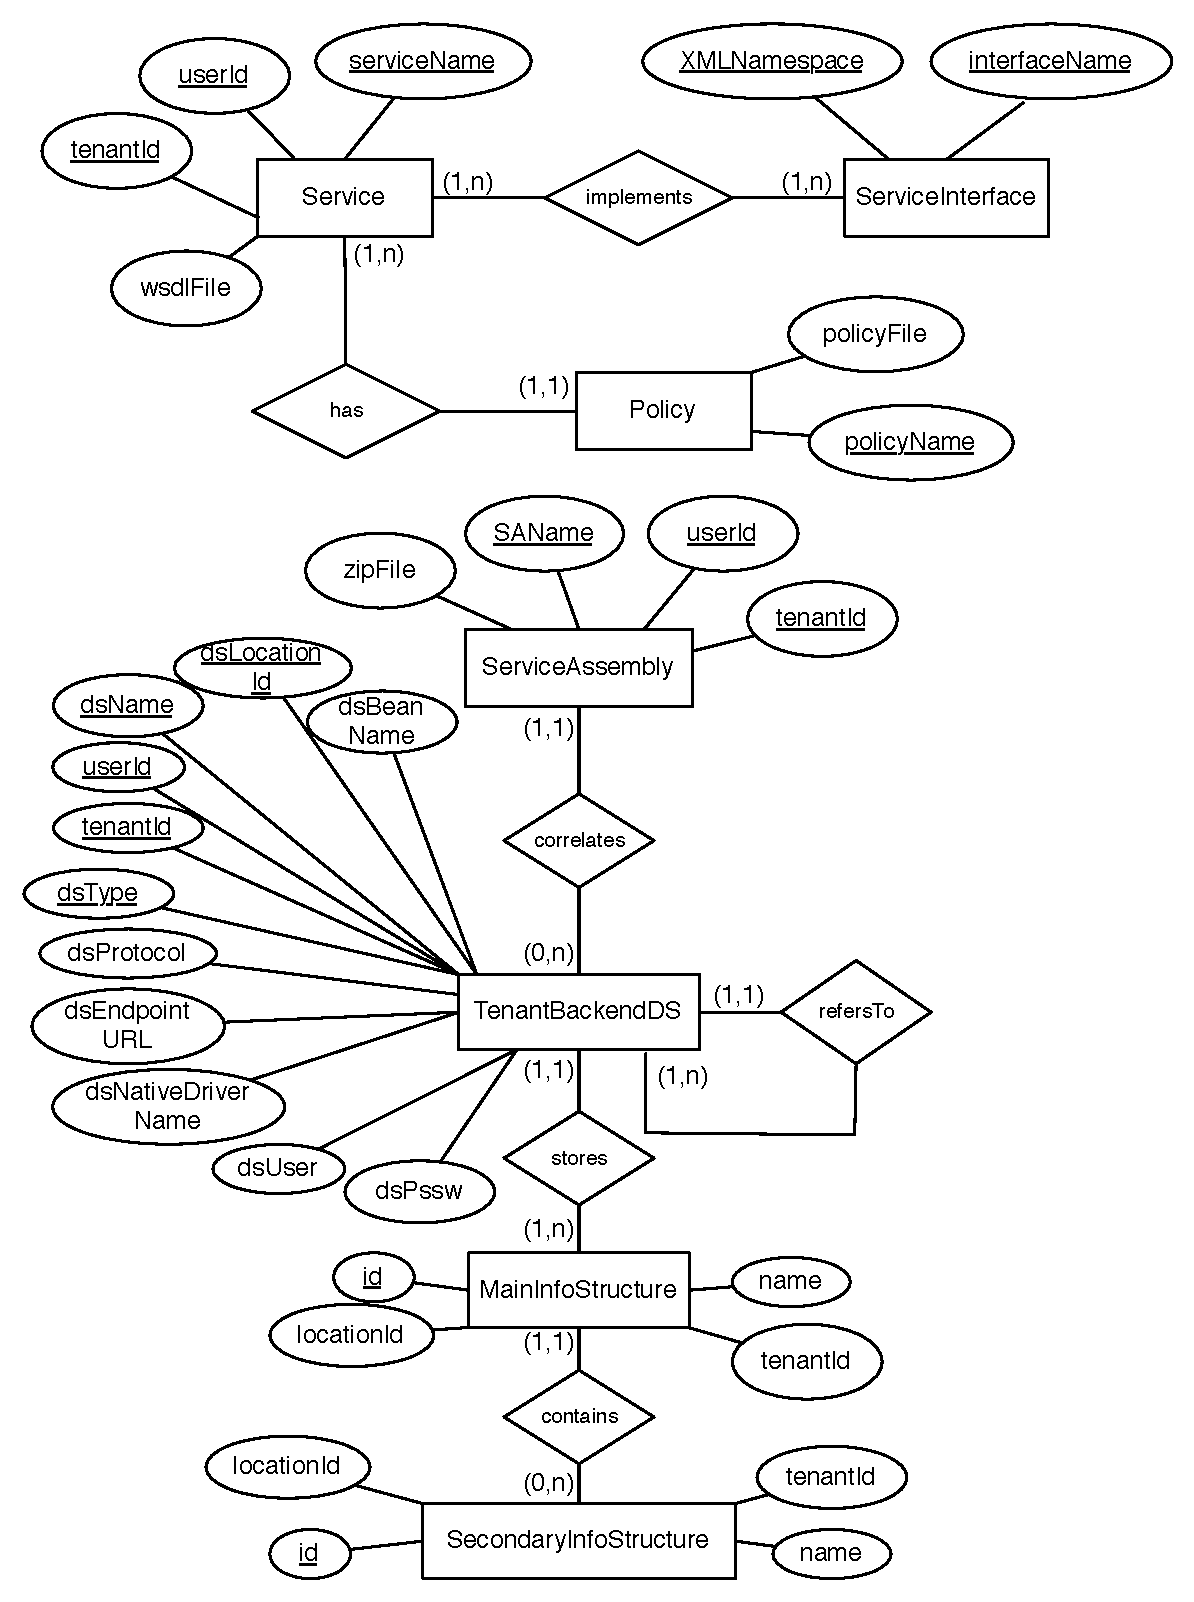
\includegraphics[clip, scale=0.7]{./gfx/dbModification/serviceRegistryV5_0_doc.pdf}
	\caption[Service Registry ER Diagram]{Extended service registry ER Diagram using (Min, Max) notation. Note: extended from outputs in \cite{Muhler2012} and \cite{Uralov2012}}
	\label{fig:serviceregistry}
\end{figure}

The service registry developed in Muhler's approach \cite{Muhler2012}, and extended in Uralov's work \cite{Uralov2012}, contains information related to the services, and policies which can be dynamically retrieved by the tenants. The services contains a WSDL file and implements an interface for its access. Furthermore, policies are attached to it in order to provide a dynamic discovery of services based on a set of rules. In this diploma thesis, we do not focus on service registering or service discovery, but on the endpoint configurations which are deployed by the tenants. These are stored in the service assembly entity, where the deployed \ac{SA}s are persisted with tenant context information. 

A \ac{SA} contains the \ac{SU}s where the endpoint configuration is described. Therefore, we consider the service assembly entity as the start point of our extension in the service registry schema. We use the data sources name to refer to the user's data sources, and categorize them as source or target data sources in the \term{dsLocationId} attribute. The  data source name in source data source registrations must equal to the database name the user includes in his request to CDASMix. Source data sources are the ones the tenant physically accesses in our system, while the target data sources are the ones that the tenant logically accesses, but the system physically accesses. Physical location of the target data sources are described in the \term{dsEndpointURL}, and define the database endpoint's host, port, and database name (an example is provided in Listing \ref{lst:testaddds}). A \ac{SA} contains the routing information configuration for routing operations between endpoints. Hence, one service assembly identifies the tenant's user source data sources. The source datasource can be connected to one or more target data sources, as shown in Figure \ref{fig:serviceregistry}. The self-referencing relation in the TenantBackendDS entity allows to reference one source data source with n target data sources.

As discussed in Chapter \ref{chap:relatedworks}, providing support for two different databases models, and for its different families (e.g. in \ac{NoSQL} databases) forces us to dissect their storage structures, and provide a generic and extensible model in order to store its meta-data. The \ac{SQL} data stores have two main storage structures: database and table. Inside the table we find a second storage structure, rows and columns. The \ac{NoSQL} databases are divided into different families, and for each family we find between the different vendors different namings which refer to the same storage structure. However, they all have in common the support of a main, and secondary storage structures. 

The data source entity stores the necessary information for providing access in the system, and for accessing the target databases in the target data sources. The configuration information is provided either by the tenant, or by the \term{Cloud Data Migration Application}, during and/or after the data migration process to the Cloud. We provide isolation in the registration of sensible information, e.g. access credentials, by indexing the table with the tenant and user \ac{UUID}. Whether transformation operations are required is detected by analyzing the value contained in the \term{dsType} attribute. The format of its value must comply the following standard: family-mainInfoStructure-secInfoStructure-version, e.g. sql-database-table-mysql5.1.2 for a MySQL database system, or nosqlKeyValue-bucket-object-1.0 for a bucket in Google Cloud Storage \cite{mysqlmanual}, \cite{googlecloudstorage}.  

The main information structure entity persists the data related to the database's main storage structure, e.g. table in MySQL databases, and table, bucket, or domain in \ac{NoSQL} databases. These storage structures are identified by its name in the backend data store. The locationid attribute in this entity categorizes one main information structure as source or target main information structure. A composite key formed by the name, locationid, and tenantid, is not possible in this entity. One tenant id may have the same name to identify two main information structure which are of a different database type, e.g. one \ac{SQL} table, and one \ac{NoSQL} bucket with the same name. Therefore, the entries in this entity are identified by a incremental id.   

The secondary information structure is used in our system only to persist meta-data for \ac{NoSQL} databases. The knowledge level in the system of tenant's migrated \ac{SQL} databases lowers to the table storage structure, and one database is uniquely associated with one tenant, user, and endpoint in the target database system, e.g in Amazon RDS one database is accessed by the database instance identifier, and the host name \cite{amazonrds}. However, different main storage structures can be accessed in \ac{NoSQL} databases through the same user's endpoint. Therefore, we need to persist one or more main storage structures per database system endpoint, and provide a second level, the secondary information structure, to register a tenant's \ac{NoSQL} database meta-data. For example, one tenant can create one or more buckets in the Google Cloud Storage system, and access them through the same endpoint \cite{googlecloudstorage}. Buckets store one or more objects, which are identified by their name. We must then associate a tenant's \ac{NoSQL} data store with one or more buckets, and these with one or more objects. A composite key formed by the name, tenantid, and locationid, is not possible, for the same reason discussed previously. One tenant id may have the same name to identify two secondary information structure which are of a different \ac{NoSQL} database type, e.g. one document, and one object with the same name. Therefore, the entries in this entity are identified by a incremental id.  As the relationships between secondary and main information structure, main information structure and data source, and between data sources (source and target) are a one to one relation, we avoid with the cascade option deleting   information which might be related with multiple entities, e.g. one target data source which is associated with two source data sources. 

The entities related to the upper entities, e.g. a second information structure related to a main information structure, and this to a data source, and to a service assembly, are set with the Java persistence property \term{Cascade}. The service assembly is the upper entity which defines the connection between one source, and multiple target data sources. The undeployment of a service assembly involves the deletion of the data sources which are related to the service assembly, and the main and secondary information structures. 

\FloatBarrier